\section{Packages Common e config}
I package contengono i seguenti file .java:

\begin{figure}[H] 
    \centering 
    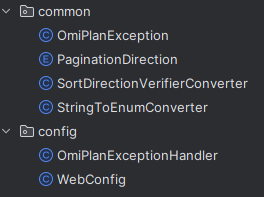
\includegraphics[width=0.4\columnwidth]{common-config} 
    \caption{Package common e config}
\end{figure}
\subsection{Common}
\begin{itemize}
\item \texttt{OmiPlanException}, eccezione personalizzata utilizzata per gestire le \textit{RuntimeException}. Classe formata da un HttpStatus per mostrare lo stato di risposta HTTP e dal messaggio fornito al lancio dell'eccezione;
\item \texttt{PaginationDirection}, classe enumerativa per gestire la direzione della paginazione\textsubscript{g} (ASC o DESC);
\item \texttt{SortDirectionVerifierConverter}, classe che implementa l'interfaccia \textit{Converter<S,T>} (componente Java utilizzato quando si lavora con strutture dati o oggetti che devono essere trasformati o adattatati in tipi diversi) per verificare che la direzione inserita sia ASC o DESC e gestire la \textit{RunTimeException} in caso non sia una variabile enum;
\item \texttt{StringToEnumConverter}, classe che implementa l'interfaccia \textit{Converter<S,T>} per convertire la direzione Stringa inserita nell'enum della direzione di pagina.
\end{itemize}

\subsection{Config}
\begin{itemize}
\item \texttt{OmiPlanExceptionHandler}, handler con il compito di gestire le eccezioni runtime, segnando quelle non gestite come "Unexpected error". Questa classe è annotata con \textit{@ControllerAdvice}, poiché definisce una classe che gestisce in maniera centralizzata le eccezioni. Contiene due metodi annotati con \textit{@ExceptionHandler} che gestiscono rispettivamente le \textit{RunTimeException} e le altre eccezioni \textit{Exception};
\item \texttt{WebConfig}, classe annotata con l'annotazione \textit{@Configuration} indicando che è una classe di configurazione e che contiene definizioni di bean o altre configurazioni necessarie per l'applicazione. Essa infatti estende \textit{WebMvcConfigurer} che consente di modificare le configurazioni predefinite di Spring MVC, in questo caso aggiungendo i converter sopra citati.
\end{itemize}